我々はまず小さいハンドル教師データを学習した結果で,
ランダムの初期配置によって8台ロボット対面走行を実験した.
Fig.\ref{handle15_dia}は時間($s$横軸)と$\theta$(縦軸上),$R$(縦軸下)の関係図です.
この実験から,一部のロボット達が短時間の対面走行できると確認したけど,
ロボット同士がぶつかる,壁にぶつかる,引っかかって解消不能,方向転換なども観察された.

例として,左の上から3番目,右の上から2番目と3番目のグラフで,$\theta$の変動が止まって,水平になった,
Fig.\ref{handle15_img}は約400秒$\theta$が水平になる部分に対する実験風景です,
実験からロボットが壁にぶつかって,後退しなくて,止まっちゃう,
2つロボットが引っかかって解消不能になって,止まっちゃうことが観察された.
原因として,曲がりと後退のパワーが弱いと考えて,大きいハンドルのラジコンで教師データを収集して実験した,
実験結果は次に説明する.

\vspace{-1mm}
\begin{figure}[!ht]
    \centering
    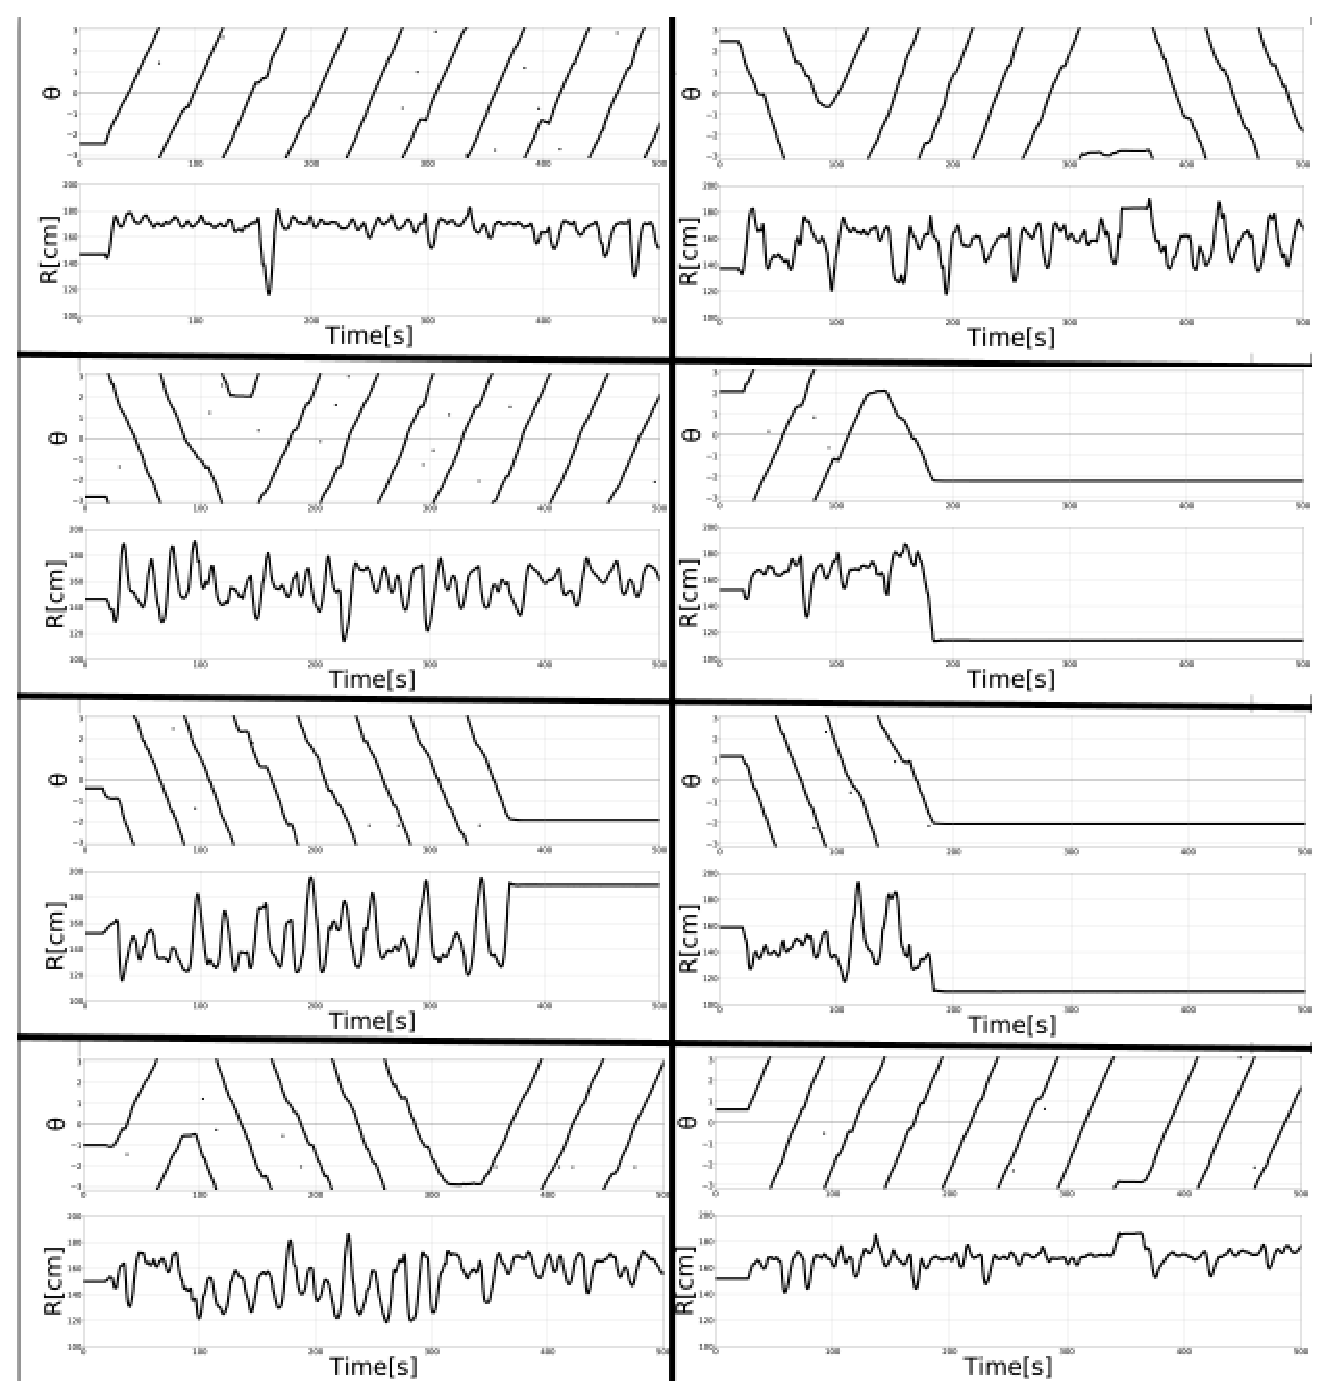
\includegraphics[width=1.0\linewidth]{NN_handle15.eps}
    \caption{小さいハンドルNN,8台ロボットの走行結果}
    \label{handle15_dia}
\end{figure}

\vspace{-5mm}
\begin{figure}[!ht]
    \centering
    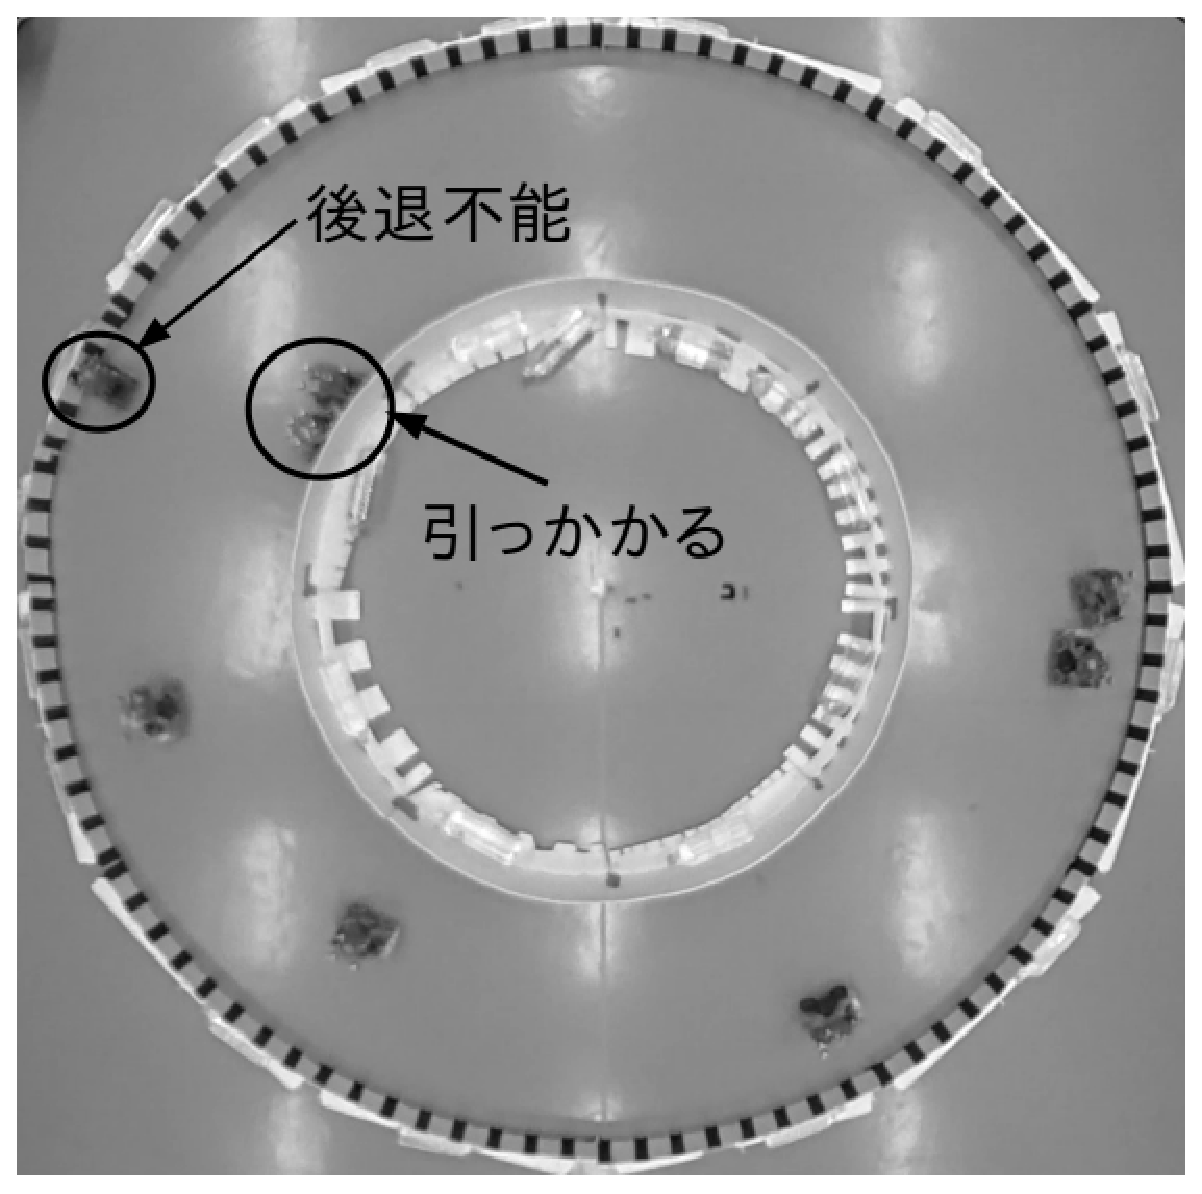
\includegraphics[width=0.6\linewidth]{nnhandle15.eps}
    \caption{小さいハンドルNN走行実験400秒の様子}
    \label{handle15_img}
\end{figure}
